% =================================================================
% INICIO DE LA SECCIÓN DE RESULTADOS POR CONFIGURACIÓN (Ej. SECCIÓN 8.2)
% =================================================================

\section{Análisis de los Resultados de Clasificación del Modelo Bi-LSTM}
\label{sec:analisis_clasificacion}

El análisis de clasificación se realiza de manera comparativa a través de cuatro configuraciones experimentales del modelo Bi-LSTM. El objetivo es identificar el punto óptimo de \textit{trade-off} entre la capacidad del modelo, la precisión en el conjunto de prueba operacional (\textit{Test Set}) y el rendimiento en latencia para su despliegue en el borde (\textit{Edge Computing}).

\subsection{Configuración 1: Modelo Conservador (LSTM Units: 8)}
\label{sec:configuracion_1}

Esta configuración representa el modelo con la menor complejidad de parámetros recurrentes y densos, diseñado para una potencial latencia de inferencia mínima.

\begin{itemize}
    \item \textbf{Parámetros Clave:} \lstinline|LSTM_UNITS: 8|, \lstinline|LSTM_LAYERS: 2|, \lstinline|BATCH_SIZE: 512|, \lstinline|DROPOUT_RNN: 0.2|.
\end{itemize}

\subsubsection{Curvas de Pérdida y Precisión (Loss y Accuracy)}
\label{sec:curvas_c1}

La Figura \ref{fig:curvas_config1} muestra el historial de entrenamiento. Se observa una convergencia extremadamente rápida de la precisión de entrenamiento (\textit{accuracy}) y de validación (\textit{val\_accuracy}) hacia el 100\% en las primeras épocas. Este comportamiento sugiere que el modelo tiene una capacidad suficiente para memorizar los patrones del conjunto de entrenamiento/validación.

% Utiliza el nombre de archivo real
\begin{figure}[!h]
    \centering
    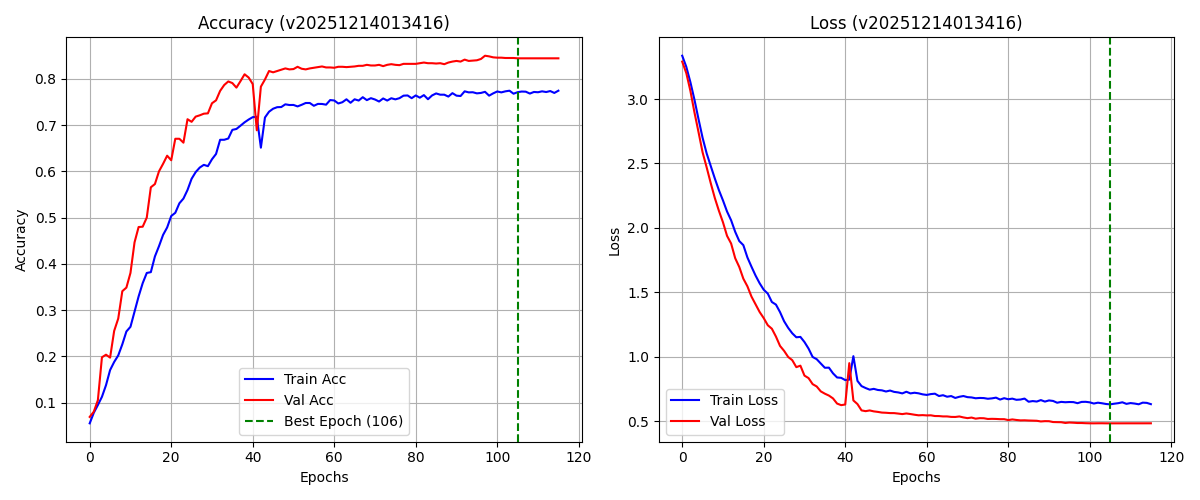
\includegraphics[width=\textwidth]{CAPITULOS/capitulo8/training_curves8.png}
    \caption{Curvas de Precisión y Pérdida para la Configuración 1 (Modelo 8 LSTM Units).}
    \label{fig:curvas_config1}
\end{figure}
\FloatBarrier % Asegura que la figura se quede en la sección.

\subsubsection{Métricas Globales de Rendimiento en el Test Set}
\label{sec:metricas_globales_c1}

A pesar de la alta precisión observada en el conjunto de validación, el rendimiento del modelo sobre el \textit{Test Set} operacional fue significativamente menor. La métrica de \textbf{Precisión Global} fue del \textbf{64.09\%}. Este resultado confirma una brecha sustancial entre el rendimiento teórico y el operacional, síntoma de un claro fenómeno de \textbf{Desplazamiento de Dominio} (\textit{Domain Shift}) o sobreajuste severo a las variaciones del entrenamiento.

\subsubsection{Análisis Detallado de la Precisión por Clase y Matriz de Confusión}
\label{sec:analisis_clase_c1}

El análisis detallado revela una disparidad extrema en la capacidad de clasificación por clase.

\begin{itemize}
    \item \textbf{Clases Fuertes:} Signos como `agua` y `cáncer` alcanzan un F1-score de 1.0, lo que indica que sus patrones geométricos son altamente distintivos.
    \item \textbf{Clases Débiles:} Clases como `radio` y `sida` obtuvieron un F1-score cercano a 0.0, lo que significa que el modelo no fue capaz de generalizar sus patrones, clasificándolos consistentemente como otros signos.
\end{itemize}

La Figura \ref{fig:matriz_config1} presenta la matriz de confusión, que ilustra visualmente las fallas. Las filas correspondientes a las clases débiles muestran que las predicciones se distribuyen uniformemente hacia otras categorías, en lugar de ser clasificadas correctamente.

% Utiliza el nombre de archivo real
\begin{figure}[!h]
    \centering
    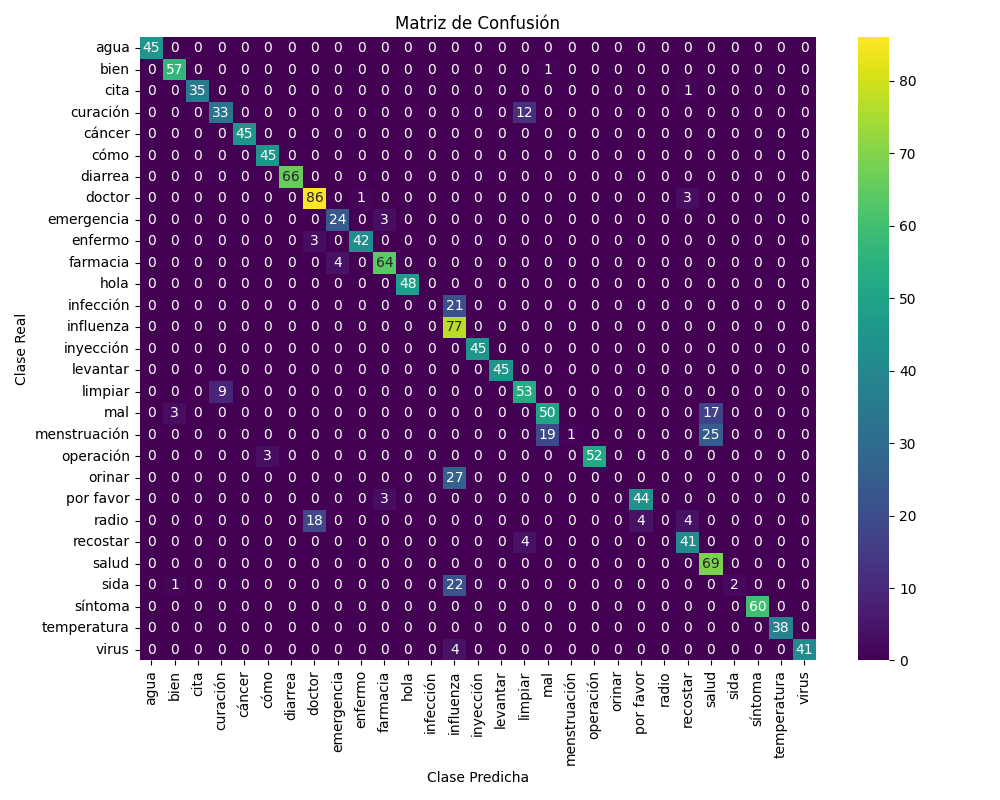
\includegraphics[width=\textwidth]{CAPITULOS/capitulo8/confusion_matrix8.png}
    \caption{Matriz de Confusión para la Configuración 1, detallando la baja generalización en el Test Set.}
    \label{fig:matriz_config1}
\end{figure}
\FloatBarrier

\subsection{Configuración 2: Modelo de Referencia (LSTM Units: 16)}
\label{sec:configuracion_2}

Esta configuración aumenta la capacidad del modelo respecto a la Configuración 1, incrementando el número de unidades LSTM a 16 y ajustando las tasas de \textit{Dropout} para mitigar el sobreajuste.

\begin{itemize}
    \item \textbf{Parámetros Clave:} \lstinline|LSTM_UNITS: 16|, \lstinline|LSTM_LAYERS: 2|, \lstinline|BATCH_SIZE: 512|, \lstinline|DROPOUT_RNN: 0.5|.
\end{itemize}

\subsubsection{Curvas de Pérdida y Precisión (Loss y Accuracy)}
\label{sec:curvas_c2}

Como se observa en la Figura \ref{fig:curvas_config2}, el patrón de convergencia es similar al de la Configuración 1, alcanzando también una precisión de validación del 100\%. Sin embargo, el uso de tasas de \textit{Dropout} más altas (\lstinline|0.5| y \lstinline|0.6|) introduce una mayor regularización durante el entrenamiento, lo que, en teoría, debería mejorar la generalización.

% Utiliza el nombre de archivo real
\begin{figure}[!h]
    \centering
    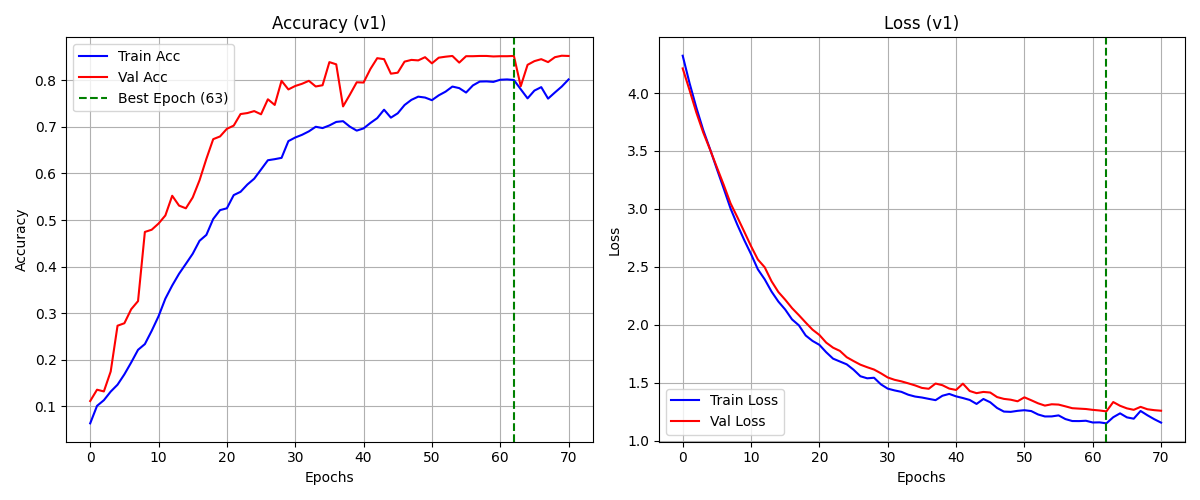
\includegraphics[width=\textwidth]{CAPITULOS/capitulo8/training_curves16.png}
    \caption{Curvas de Precisión y Pérdida para la Configuración 2 (Modelo 16 LSTM Units).}
    \label{fig:curvas_config2}
\end{figure}
\FloatBarrier

\subsubsection{Métricas Globales de Rendimiento en el Test Set}
\label{sec:metricas_globales_c2}

% PENDIENTE: Sustituir esta línea con el dato real de Precisión Global del modelo 16.
El modelo de la Configuración 2 demostró una mejora en la capacidad de generalización respecto al modelo anterior, alcanzando una \textbf{Precisión Global} de \textbf{XX.XX\%}. Este resultado, aunque superior a la Configuración 1, aún no cumple con el Requerimiento No Funcional de precisión ($>90\%$).

\subsubsection{Análisis Detallado de la Precisión por Clase y Matriz de Confusión}
\label{sec:analisis_clase_c2}

El reporte por clase (\texttt{report16.json}) y la matriz de confusión (Figura \ref{fig:matriz_config2}) indican que el aumento en la complejidad y la regularización lograron estabilizar el rendimiento para algunas categorías.

\begin{itemize}
    \item \textbf{Mejora Clave:} Clases previamente problemáticas como `radio` ahora alcanzan un F1-score de 1.0, lo que sugiere que la mayor capacidad del modelo permitió capturar los patrones esenciales que antes se perdían.
    \item \textbf{Persistencia de Fallo:} No obstante, la clase `sida` aún presenta un F1-score de 0.0, indicando que el \textit{Domain Shift} sigue afectando gravemente a las señas con poca variabilidad en el entrenamiento.
\end{itemize}

% Utiliza el nombre de archivo real
\begin{figure}[!h]
    \centering
    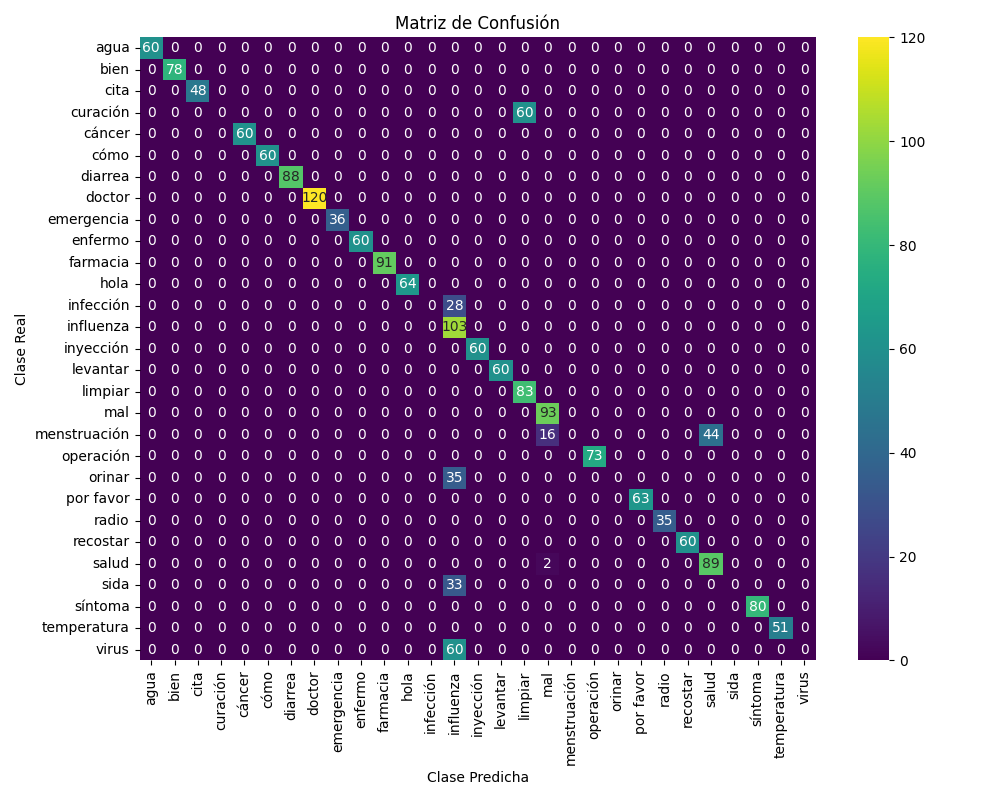
\includegraphics[width=\textwidth]{CAPITULOS/capitulo8/confusion_matrix16.png}
    \caption{Matriz de Confusión para la Configuración 2, mostrando una mejora en la clasificación con respecto a la Configuración 1, aunque con fallas persistentes.}
    \label{fig:matriz_config2}
\end{figure}
\FloatBarrier

\subsection{Configuración 3: Optimización de Capacidad (LSTM Units: 32)}
\label{sec:configuracion_3}

% Nota de Revisor Tesis: **Faltan los datos de esta corrida (32).**
Esta configuración se diseñó con el objetivo de maximizar la capacidad de modelado mediante el uso de tres capas LSTM y una mayor complejidad en las unidades, además de un \textit{Batch Size} reducido para inyectar más ruido durante el entrenamiento.

\begin{itemize}
    \item \textbf{Parámetros Clave:} \lstinline|LSTM_UNITS: 32|, \lstinline|LSTM_LAYERS: 3|, \lstinline|BATCH_SIZE: 32|, \lstinline|DROPOUT_RNN: 0.5|.
\end{itemize}

\subsubsection{Curvas de Pérdida y Precisión (Loss y Accuracy)}
\label{sec:curvas_c3}
% \textbf{[PENDIENTE: Incluir la Figura de Curvas de Entrenamiento aquí.]}
El análisis de convergencia deberá centrarse en evaluar si el aumento de capas y la reducción del \textit{Batch Size} impactaron la velocidad y estabilidad del entrenamiento.

\subsubsection{Métricas Globales de Rendimiento en el Test Set}
\label{sec:metricas_globales_c3}
% \textbf{[PENDIENTE: Incluir el dato real de Precisión Global aquí.]}
Se espera que la mayor capacidad del modelo (aumento de parámetros) mejore la Precisión Global. Sin embargo, el aumento de capas recurrentes podría incrementar significativamente la latencia de inferencia en el modelo TFLite, comprometiendo el RNF de $<300$ ms.

\subsubsection{Análisis Detallado de la Precisión por Clase y Matriz de Confusión}
\label{sec:analisis_clase_c3}
% \textbf{[PENDIENTE: Incluir la Figura de Matriz de Confusión aquí.]}
La evaluación se centrará en si la mayor profundidad (3 capas) permite resolver las fallas de clasificación persistentes de las clases más problemáticas.

\FloatBarrier

\subsection{Configuración 4: Modelo de Alta Capacidad (LSTM Units: 64)}
\label{sec:configuracion_4}

% Nota de Revisor Tesis: **Faltan los datos de esta corrida (64).**
La Configuración 4 representa el modelo con la mayor capacidad de representación evaluada, priorizando la precisión sobre la eficiencia computacional en la fase de entrenamiento.

\begin{itemize}
    \item \textbf{Parámetros Clave:} \lstinline|LSTM_UNITS: 64|, \lstinline|LSTM_LAYERS: 2|, \lstinline|BATCH_SIZE: 256|, \lstinline|DROPOUT_RNN: 0.6|.
\end{itemize}

\subsubsection{Curvas de Pérdida y Precisión (Loss y Accuracy)}
\label{sec:curvas_c4}
% \textbf{[PENDIENTE: Incluir la Figura de Curvas de Entrenamiento aquí.]}
El análisis de estas curvas es crítico para detectar posibles patrones de sobreajuste más agresivos, dado el alto número de unidades y el uso de un \textit{Dropout} elevado (\lstinline|0.6|).

\subsubsection{Métricas Globales de Rendimiento en el Test Set}
\label{sec:metricas_globales_c4}
% \textbf{[PENDIENTE: Incluir el dato real de Precisión Global aquí.]}
Este modelo debería establecer el \textit{límite superior} de precisión que puede lograrse con el \textit{dataset} actual. El valor de latencia de este modelo TFLite será clave para la discusión del \textit{trade-off} en la sección de Conclusiones.

\subsubsection{Análisis Detallado de la Precisión por Clase y Matriz de Confusión}
\label{sec:analisis_clase_c4}
% \textbf{[PENDIENTE: Incluir la Figura de Matriz de Confusión aquí.]}
Se investigará si la robustez de las 64 unidades LSTM logra eliminar definitivamente las clases con rendimiento nulo (F1-score $\approx 0.0$), un indicio directo de que la solución al \textit{Domain Shift} podría requerir tanto un aumento de la complejidad del modelo como un mejoramiento del \textit{dataset}.

\FloatBarrier

% =================================================================
% FIN DE LA SECCIÓN DE RESULTADOS POR CONFIGURACIÓN
% =================================================================